% Options for packages loaded elsewhere
% Options for packages loaded elsewhere
\PassOptionsToPackage{unicode}{hyperref}
\PassOptionsToPackage{hyphens}{url}
\PassOptionsToPackage{dvipsnames,svgnames,x11names}{xcolor}
%
\documentclass[
  letterpaper,
  DIV=11,
  numbers=noendperiod]{scrreprt}
\usepackage{xcolor}
\usepackage{amsmath,amssymb}
\setcounter{secnumdepth}{5}
\usepackage{iftex}
\ifPDFTeX
  \usepackage[T1]{fontenc}
  \usepackage[utf8]{inputenc}
  \usepackage{textcomp} % provide euro and other symbols
\else % if luatex or xetex
  \usepackage{unicode-math} % this also loads fontspec
  \defaultfontfeatures{Scale=MatchLowercase}
  \defaultfontfeatures[\rmfamily]{Ligatures=TeX,Scale=1}
\fi
\usepackage{lmodern}
\ifPDFTeX\else
  % xetex/luatex font selection
\fi
% Use upquote if available, for straight quotes in verbatim environments
\IfFileExists{upquote.sty}{\usepackage{upquote}}{}
\IfFileExists{microtype.sty}{% use microtype if available
  \usepackage[]{microtype}
  \UseMicrotypeSet[protrusion]{basicmath} % disable protrusion for tt fonts
}{}
\makeatletter
\@ifundefined{KOMAClassName}{% if non-KOMA class
  \IfFileExists{parskip.sty}{%
    \usepackage{parskip}
  }{% else
    \setlength{\parindent}{0pt}
    \setlength{\parskip}{6pt plus 2pt minus 1pt}}
}{% if KOMA class
  \KOMAoptions{parskip=half}}
\makeatother
% Make \paragraph and \subparagraph free-standing
\makeatletter
\ifx\paragraph\undefined\else
  \let\oldparagraph\paragraph
  \renewcommand{\paragraph}{
    \@ifstar
      \xxxParagraphStar
      \xxxParagraphNoStar
  }
  \newcommand{\xxxParagraphStar}[1]{\oldparagraph*{#1}\mbox{}}
  \newcommand{\xxxParagraphNoStar}[1]{\oldparagraph{#1}\mbox{}}
\fi
\ifx\subparagraph\undefined\else
  \let\oldsubparagraph\subparagraph
  \renewcommand{\subparagraph}{
    \@ifstar
      \xxxSubParagraphStar
      \xxxSubParagraphNoStar
  }
  \newcommand{\xxxSubParagraphStar}[1]{\oldsubparagraph*{#1}\mbox{}}
  \newcommand{\xxxSubParagraphNoStar}[1]{\oldsubparagraph{#1}\mbox{}}
\fi
\makeatother

\usepackage{color}
\usepackage{fancyvrb}
\newcommand{\VerbBar}{|}
\newcommand{\VERB}{\Verb[commandchars=\\\{\}]}
\DefineVerbatimEnvironment{Highlighting}{Verbatim}{commandchars=\\\{\}}
% Add ',fontsize=\small' for more characters per line
\usepackage{framed}
\definecolor{shadecolor}{RGB}{241,243,245}
\newenvironment{Shaded}{\begin{snugshade}}{\end{snugshade}}
\newcommand{\AlertTok}[1]{\textcolor[rgb]{0.68,0.00,0.00}{#1}}
\newcommand{\AnnotationTok}[1]{\textcolor[rgb]{0.37,0.37,0.37}{#1}}
\newcommand{\AttributeTok}[1]{\textcolor[rgb]{0.40,0.45,0.13}{#1}}
\newcommand{\BaseNTok}[1]{\textcolor[rgb]{0.68,0.00,0.00}{#1}}
\newcommand{\BuiltInTok}[1]{\textcolor[rgb]{0.00,0.23,0.31}{#1}}
\newcommand{\CharTok}[1]{\textcolor[rgb]{0.13,0.47,0.30}{#1}}
\newcommand{\CommentTok}[1]{\textcolor[rgb]{0.37,0.37,0.37}{#1}}
\newcommand{\CommentVarTok}[1]{\textcolor[rgb]{0.37,0.37,0.37}{\textit{#1}}}
\newcommand{\ConstantTok}[1]{\textcolor[rgb]{0.56,0.35,0.01}{#1}}
\newcommand{\ControlFlowTok}[1]{\textcolor[rgb]{0.00,0.23,0.31}{\textbf{#1}}}
\newcommand{\DataTypeTok}[1]{\textcolor[rgb]{0.68,0.00,0.00}{#1}}
\newcommand{\DecValTok}[1]{\textcolor[rgb]{0.68,0.00,0.00}{#1}}
\newcommand{\DocumentationTok}[1]{\textcolor[rgb]{0.37,0.37,0.37}{\textit{#1}}}
\newcommand{\ErrorTok}[1]{\textcolor[rgb]{0.68,0.00,0.00}{#1}}
\newcommand{\ExtensionTok}[1]{\textcolor[rgb]{0.00,0.23,0.31}{#1}}
\newcommand{\FloatTok}[1]{\textcolor[rgb]{0.68,0.00,0.00}{#1}}
\newcommand{\FunctionTok}[1]{\textcolor[rgb]{0.28,0.35,0.67}{#1}}
\newcommand{\ImportTok}[1]{\textcolor[rgb]{0.00,0.46,0.62}{#1}}
\newcommand{\InformationTok}[1]{\textcolor[rgb]{0.37,0.37,0.37}{#1}}
\newcommand{\KeywordTok}[1]{\textcolor[rgb]{0.00,0.23,0.31}{\textbf{#1}}}
\newcommand{\NormalTok}[1]{\textcolor[rgb]{0.00,0.23,0.31}{#1}}
\newcommand{\OperatorTok}[1]{\textcolor[rgb]{0.37,0.37,0.37}{#1}}
\newcommand{\OtherTok}[1]{\textcolor[rgb]{0.00,0.23,0.31}{#1}}
\newcommand{\PreprocessorTok}[1]{\textcolor[rgb]{0.68,0.00,0.00}{#1}}
\newcommand{\RegionMarkerTok}[1]{\textcolor[rgb]{0.00,0.23,0.31}{#1}}
\newcommand{\SpecialCharTok}[1]{\textcolor[rgb]{0.37,0.37,0.37}{#1}}
\newcommand{\SpecialStringTok}[1]{\textcolor[rgb]{0.13,0.47,0.30}{#1}}
\newcommand{\StringTok}[1]{\textcolor[rgb]{0.13,0.47,0.30}{#1}}
\newcommand{\VariableTok}[1]{\textcolor[rgb]{0.07,0.07,0.07}{#1}}
\newcommand{\VerbatimStringTok}[1]{\textcolor[rgb]{0.13,0.47,0.30}{#1}}
\newcommand{\WarningTok}[1]{\textcolor[rgb]{0.37,0.37,0.37}{\textit{#1}}}

\usepackage{longtable,booktabs,array}
\newcounter{none} % for unnumbered tables
\usepackage{calc} % for calculating minipage widths
% Correct order of tables after \paragraph or \subparagraph
\usepackage{etoolbox}
\makeatletter
\patchcmd\longtable{\par}{\if@noskipsec\mbox{}\fi\par}{}{}
\makeatother
% Allow footnotes in longtable head/foot
\IfFileExists{footnotehyper.sty}{\usepackage{footnotehyper}}{\usepackage{footnote}}
\makesavenoteenv{longtable}
\usepackage{graphicx}
\makeatletter
\newsavebox\pandoc@box
\newcommand*\pandocbounded[1]{% scales image to fit in text height/width
  \sbox\pandoc@box{#1}%
  \Gscale@div\@tempa{\textheight}{\dimexpr\ht\pandoc@box+\dp\pandoc@box\relax}%
  \Gscale@div\@tempb{\linewidth}{\wd\pandoc@box}%
  \ifdim\@tempb\p@<\@tempa\p@\let\@tempa\@tempb\fi% select the smaller of both
  \ifdim\@tempa\p@<\p@\scalebox{\@tempa}{\usebox\pandoc@box}%
  \else\usebox{\pandoc@box}%
  \fi%
}
% Set default figure placement to htbp
\def\fps@figure{htbp}
\makeatother

\ifLuaTeX
  \usepackage{luacolor}
  \usepackage[soul]{lua-ul}
\else
  \usepackage{soul}
\fi




\setlength{\emergencystretch}{3em} % prevent overfull lines

\providecommand{\tightlist}{%
  \setlength{\itemsep}{0pt}\setlength{\parskip}{0pt}}



 


% preamble.tex

% Language / paragraph style
\usepackage[english]{babel}
\setlength{\parindent}{0pt}

% Core packages
\usepackage{booktabs}
\usepackage{array}
\usepackage{amsmath}
\usepackage{graphicx}
\usepackage{float}
\usepackage[most]{tcolorbox}
\usepackage{pdflscape}
\usepackage{lipsum}
\usepackage{longtable}
\usepackage{caption}
\usepackage{multirow}
\usepackage{rotating}

% Fonts: Arial-like / Calibri-like via XeLaTeX
\usepackage{fontspec}
\setmainfont{Arial}
\setsansfont{Arial}

% If Arial fails on your machine, replace both lines above with:
% \setmainfont{TeX Gyre Heros}
% \setsansfont{TeX Gyre Heros}

% Custom column types
\newcolumntype{L}[1]{>{\raggedright\arraybackslash}p{#1}}
\newcolumntype{C}[1]{>{\centering\arraybackslash}p{#1}}

% Page geometry
\usepackage[
  a4paper,
  top=1.5in,
  bottom=1in,
  left=1in,
  right=1in,
  headheight=75pt,
  headsep=15pt
]{geometry}

% Header / footer
\usepackage{fancyhdr}
\pagestyle{fancy}
\fancyhf{}
\renewcommand{\headrulewidth}{0pt}

\fancyhead[C]{%
  \makebox[\textwidth]{%
    
\includegraphics[height=35pt]{resources/rufas.png}\hfill
    \textbf{\today}%
  }\\
  \textbf{Scientific Documentation of RuFaS Model}\\
  \rule{\textwidth}{1pt}
}

\renewcommand{\footrulewidth}{0.4pt}
\fancyfoot[L]{%
  \begin{tabular}[t]{@{}l@{}}
    Ruminant Farm System\\
    Sci Doc v.1
  \end{tabular}%
}
\fancyfoot[C]{\thepage}
\fancyfoot[R]{\nouppercase{\leftmark}}

\fancypagestyle{landscapeplain}{
  \fancyhf{}
  \renewcommand{\headrulewidth}{0pt}
  \renewcommand{\footrulewidth}{0pt}
}
\KOMAoption{captions}{tableheading}
\makeatletter
\@ifpackageloaded{tcolorbox}{}{\usepackage[skins,breakable]{tcolorbox}}
\@ifpackageloaded{fontawesome5}{}{\usepackage{fontawesome5}}
\definecolor{quarto-callout-color}{HTML}{909090}
\definecolor{quarto-callout-note-color}{HTML}{0758E5}
\definecolor{quarto-callout-important-color}{HTML}{CC1914}
\definecolor{quarto-callout-warning-color}{HTML}{EB9113}
\definecolor{quarto-callout-tip-color}{HTML}{00A047}
\definecolor{quarto-callout-caution-color}{HTML}{FC5300}
\definecolor{quarto-callout-color-frame}{HTML}{acacac}
\definecolor{quarto-callout-note-color-frame}{HTML}{4582ec}
\definecolor{quarto-callout-important-color-frame}{HTML}{d9534f}
\definecolor{quarto-callout-warning-color-frame}{HTML}{f0ad4e}
\definecolor{quarto-callout-tip-color-frame}{HTML}{02b875}
\definecolor{quarto-callout-caution-color-frame}{HTML}{fd7e14}
\makeatother
\makeatletter
\@ifpackageloaded{bookmark}{}{\usepackage{bookmark}}
\makeatother
\makeatletter
\@ifpackageloaded{caption}{}{\usepackage{caption}}
\AtBeginDocument{%
\ifdefined\contentsname
  \renewcommand*\contentsname{Table of contents}
\else
  \newcommand\contentsname{Table of contents}
\fi
\ifdefined\listfigurename
  \renewcommand*\listfigurename{List of Figures}
\else
  \newcommand\listfigurename{List of Figures}
\fi
\ifdefined\listtablename
  \renewcommand*\listtablename{List of Tables}
\else
  \newcommand\listtablename{List of Tables}
\fi
\ifdefined\figurename
  \renewcommand*\figurename{Figure}
\else
  \newcommand\figurename{Figure}
\fi
\ifdefined\tablename
  \renewcommand*\tablename{Table}
\else
  \newcommand\tablename{Table}
\fi
}
\@ifpackageloaded{float}{}{\usepackage{float}}
\floatstyle{ruled}
\@ifundefined{c@chapter}{\newfloat{codelisting}{h}{lop}}{\newfloat{codelisting}{h}{lop}[chapter]}
\floatname{codelisting}{Listing}
\newcommand*\listoflistings{\listof{codelisting}{List of Listings}}
\makeatother
\makeatletter
\makeatother
\makeatletter
\@ifpackageloaded{caption}{}{\usepackage{caption}}
\@ifpackageloaded{subcaption}{}{\usepackage{subcaption}}
\makeatother
\usepackage{bookmark}
\IfFileExists{xurl.sty}{\usepackage{xurl}}{} % add URL line breaks if available
\urlstyle{same}
\hypersetup{
  pdftitle={mybook},
  pdfauthor={Jane Doe},
  colorlinks=true,
  linkcolor={blue},
  filecolor={Maroon},
  citecolor={Blue},
  urlcolor={Blue},
  pdfcreator={LaTeX via pandoc}}


\title{mybook}
\author{Jane Doe}
\date{2021-08-18}
\begin{document}
\maketitle

\renewcommand*\contentsname{Contents}
{
\setcounter{tocdepth}{1}
\tableofcontents
}
\listoffigures
\listoftables

\bookmarksetup{startatroot}

\chapter{Preface: A Day in the Life on a RuFaS
Farm}\label{preface-a-day-in-the-life-on-a-rufas-farm}


\includegraphics[width=0.9375in,height=\textheight,keepaspectratio]{resources/rufas.png}

This document provides a high-level overview of the daily operations of
a ruminant farm, as modeled by RuFaS. The overview will be through the
eyes of Dr.~Rue Fas. One day, Dr.~Rue woke up and decided the life of a
computer scientist wasn't for her. So she bought a dairy farm, and this
is how she operates it every day.

\textbf{Feeding the Animals} Second thing in the morning, after coffee,
Dr. Rue checks the calendar to see if it's time to formulate a new
ration for her animals.

If a new ration needs to be formulated, Dr.~Rue heads over to the barn
where she keeps all her forages and feed. While there, she checks how
well all the forages are holding up. After considering the feeds
available, the quality of each one, and how much each one costs, she
decides on how productive she wants her animals to be. It is a difficult
balancing act, but eventually a ration recipe is found that will keep
the animals happy while keeping costs low and sustainability high until
the calendar says the ration recipe needs to be reformulated.

When Dr.~Rue doesn't need to formulate a new ration, she takes the last
ration recipe she made and grabs all the feed and forage the animals
need for the day out of the feed barn. If there isn't enough for the
animals, then a new ration is formulated using the steps above.

\textbf{Taking Care of the Animals} After making sure all the animals'
feed is taken care of, Dr.~Rue moves on to taking care of all the other
animal tasks. This includes milking the animals, making sure they're
healthy, getting them pregnant, and numerous other tasks.

As dawn breaks on the RuFaS farm, the animals awaken after a restful
night. Joe, the farm master, prepares a large whiteboard to track
HerdReproductionStatistics, ensuring he has all the data he needs for
the day's activities.

\emph{Daily Routine} - After leaving their pens, each animal lines up in
front of the barn. Julie, the diligent farm veterinarian, examines them
one by one. This daily check includes updates on the following areas:

\begin{itemize}
\item
  Nutrients: Each animal begins its day with a quick phosphorus
  requirement assessment. Julie records these details and updates the
  animal's phosphorus-related metrics.
\item
  Digestive System: With nutrient information in hand, Julie shifts
  focus to each animal's digestive system, estimating manure output and
  enteric methane production for that day.
\item
  Milk Production: All milking cows are assessed to gauge daily milk
  yield and milk component content (fat and protein). Any necessary
  adjustments are noted.
\item
  Animal Growth: Around midday, Julie returns to each animal to evaluate
  daily weight changes. She updates each animal's body weight
  accordingly.
\item
  Reproduction: HeiferII and Cow stage animals undergo a reproduction
  check. Julie closely monitors their reproductive progress and updates
  the HerdReproductionStatistics details on Joe's whiteboard.
\item
  Life Stage Evaluation: Once the daily routines are complete, Julie
  determines if any animal is ready to progress to the next life stage.
  Graduating animals are marked as ``graduated'' to be moved to their
  new pens. Animals that must leave the herd---due to health,
  productivity, or other issues---are labeled as ``sold'' or ``dead'' to
  be removed from the farm population.
\item
  Herd Size Maintenance: After every animal has been evaluated, Joe
  counts the herd to ensure it remains at a healthy size. If it is too
  large, he arranges the sale of some animals. If the herd is too small,
  he may opt to purchase additional heiferIIIs to keep numbers at the
  ideal level.
\item
  Herd Structure Management: Joe also manages pen assignments. Newly
  graduated or newborn animals are guided to suitable pens, while
  animals marked for removal (sold or deceased) are taken out of the
  herd and removed from the farm records.
\end{itemize}

\begin{tcolorbox}[enhanced jigsaw, arc=.35mm, bottomrule=.15mm, bottomtitle=1mm, breakable, colback=white, colbacktitle=quarto-callout-note-color!10!white, colframe=quarto-callout-note-color-frame, coltitle=black, left=2mm, leftrule=.75mm, opacityback=0, opacitybacktitle=0.6, rightrule=.15mm, title=\textcolor{quarto-callout-note-color}{\faInfo}\hspace{0.5em}{Note}, titlerule=0mm, toprule=.15mm, toptitle=1mm]

Note: if only interested in a PDF version of the documentation (no
website version), then the original LaTeX code can still be used and
processed by quarto. For example, the bullet points works as the
original LaTeX or translated into markdown syntax:

\begin{Shaded}
\begin{Highlighting}[]
\InformationTok{\textasciigrave{}\textasciigrave{}\textasciigrave{}\{latex\}}
\InformationTok{\textbackslash{}begin\{itemize\}}
\InformationTok{    \textbackslash{}item first bullet point}
\InformationTok{    \textbackslash{}item second bullet point}
\InformationTok{    \textbackslash{}item ...}
\InformationTok{\textbackslash{}end\{itemize\}}
\InformationTok{\textasciigrave{}\textasciigrave{}\textasciigrave{}}
\end{Highlighting}
\end{Shaded}

\begin{Shaded}
\begin{Highlighting}[]
\InformationTok{\textasciigrave{}\textasciigrave{}\textasciigrave{}\{markdown\}}
\SpecialStringTok{* }\NormalTok{first bullet point}
\SpecialStringTok{* }\NormalTok{second bullet point}
\SpecialStringTok{* }\NormalTok{...}
\InformationTok{\textasciigrave{}\textasciigrave{}\textasciigrave{}}
\end{Highlighting}
\end{Shaded}

\begin{itemize}
\tightlist
\item
  first bullet point
\item
  second bullet point
\item
  \ldots{}
\end{itemize}

but only the markdown works for all document types (html, pdf, word
document, presentations, e-books, etc.).

\end{tcolorbox}

\textbf{Output Reporting} At day's end, Joe and Julie review the updated
HerdReproductionStatistics on the whiteboard. Joe then compiles a
concise report summarizing the day's herd stats. He forwards this
information to the OutputManager before wrapping up another successful
day on the RuFaS farm.

\textbf{Dealing with the Manure} Once all the animal chores are
finished, Dr.~Rue moves on to handling the manure. There are a lot of
different ways that manure is collected from the animals: it is flushed
out of the milking parlor with water, some of the pens need to have it
shoveled out along with the bedding in the pen, and some pens have
grates that allow the manure to go straight into a pit beneath the barn.

There are a lot of different places where manure is processed and stored
on the farm. Dr.~Rue goes from place to place on the farm, moving the
manure from one place to the next. The manure chores are finished after
moving all of the manure into her lagoons, compost piles, and other
storages. As this final manure chore is completed, she writes down all
the information about how much manure is in all these storages, and some
information about what that manure is made of. How much water, nitrogen,
phosphorus, other solids, etc. are in each storage.

\textbf{Managing the Fields} Now that Dr.~Rue is done making sure all
the manure has been handled and stored properly, she can take care of
all the field tasks. She has a lot of fields on her farm, each with its
own unique schedule. Her field management routine starts with checking
each field's schedule to see if any of them are due to have manure
applied, and if so, how much they should have applied. After noting all
the manure that is supposed to go onto her fields, these amounts are
checked against the amounts of manure that are in her manure storage.
Dr.~Rue then applies manure to each field on the schedule that day,
trying to match the amount applied to the amount on the schedule as best
she can.

After making sure every manure item on each farm's schedule has been
taken care of for the day, the schedule for each field is rechecked, one
field at a time. In each schedule she checks to see if that field needs
to be tilled, if any chemical fertilizer needs to be applied, and if any
crops need to be planted or harvested. After all these activities are
taken care of, Mother Nature goes to work. The sun shines and rain
falls, providing the field with water and energy that grows crops and
soaks the soil. After taking care of each field one by one, Dr.~Rue
drives back to the main farm with all of the crops that she harvested on
that day.

\textbf{Storing the Feeds} Now that she is back at the barns, all the
crops that were just harvested can be stored. Fortunately she is very
organized, so all her harvested crops are separate from one another and
each has a label, indicating where it will be stored inside the feed
barn. As each feed is stored, it is labeled with the current date.
Dr.~Rue is exhausted from another long day. She goes back to the
farmhouse and rests up, preparing to do the whole thing over again
tomorrow. Her daily routine might seem repetitive, but each day is a
crucial part of the larger, continuous process that keeps her farm
running efficiently and sustainably.

\bookmarksetup{startatroot}

\chapter{Equation examples (from Animal
Documentation)}\label{equation-examples-from-animal-documentation}

\section{Nutrient Requirements of Dairy Cattle (NRC)}\label{sec-nrc}

\textbf{Energy Requirements} For details about the variables included in
each calculation, please refer to the
\href{energy\%20requirements\%20key}{energykey}.

\begin{itemize}
\item
  \textbf{\emph{Maintenance}} - The maintenance requirement is
  calculated based on metabolic body weight (body weight\(^{0.75}\)).

  \ul{Lactating and Dry Cows}

  \begin{equation}\protect\phantomsection\label{eq-nrc-cbw}{CBW = MW * 0.06275}\end{equation}

  \begin{equation}\protect\phantomsection\label{eq-nrc-cw}{ CW = {(18 + (DOP - 190) * 0.665) * (\frac{CBW}{45}),\text{if}DOP > 190.0} }\end{equation}

  \emph{Otherwise}

  \begin{equation}\protect\phantomsection\label{eq-nrc-ne-maint}{ NEmaint = 0.08 \times (BW - CW)^{0.75} }\end{equation}
\end{itemize}

\section{Reformatted equations}\label{reformatted-equations}

Equation~\ref{eq-nrc-cbw} may be visually improved by using the
\texttt{\textbackslash{}times} LaTeX command:

\[CBW = MW \times 0.06275\]

\section{Use alphanumeric equation
labels}\label{use-alphanumeric-equation-labels}

Though quarto does not allow custom cross-reference labels, you can
include your own non-CR label with the \textbackslash tag latex command.
\emph{And} the equation can still be cross-referenceable (and assigned a
dynamic equation number) by using a custom cross-reference class
(defined in \_quarto.yml):

\protect\phantomsection\label{eqn-an-nrc-2}
\[ CBW = MW * 0.06275 \tag{\textbf{AN.NRC.2}}\]

see (\textbf{eqn-an-nrc-2?})

\section{Other equation Templates}\label{other-equation-templates}

The energy balance is \(E = mc^2\).

\begin{equation}\protect\phantomsection\label{eq-energy}{
\begin{equation}
E = mc^2
\end{equation}
}\end{equation}

See Equation Equation~\ref{eq-energy}.
\begin{equation}\protect\phantomsection\label{eq-nutrient-proportion}{
\begin{equation}
\text{nutrient\_proportion\_to\_be\_removed} =
\min\left(
\frac{\text{mass\_requested\_nutrient}}{\text{manure\_nutrient\_available}},
1
\right)
\end{equation}
}\end{equation}

\bookmarksetup{startatroot}

\chapter{Animal Module}\label{animal-module}

\section{Introduction}\label{introduction}

\subsection{Example of a Figure}\label{example-of-a-figure}

This is a great example of how to set up a module.

\begin{figure}

\centering{

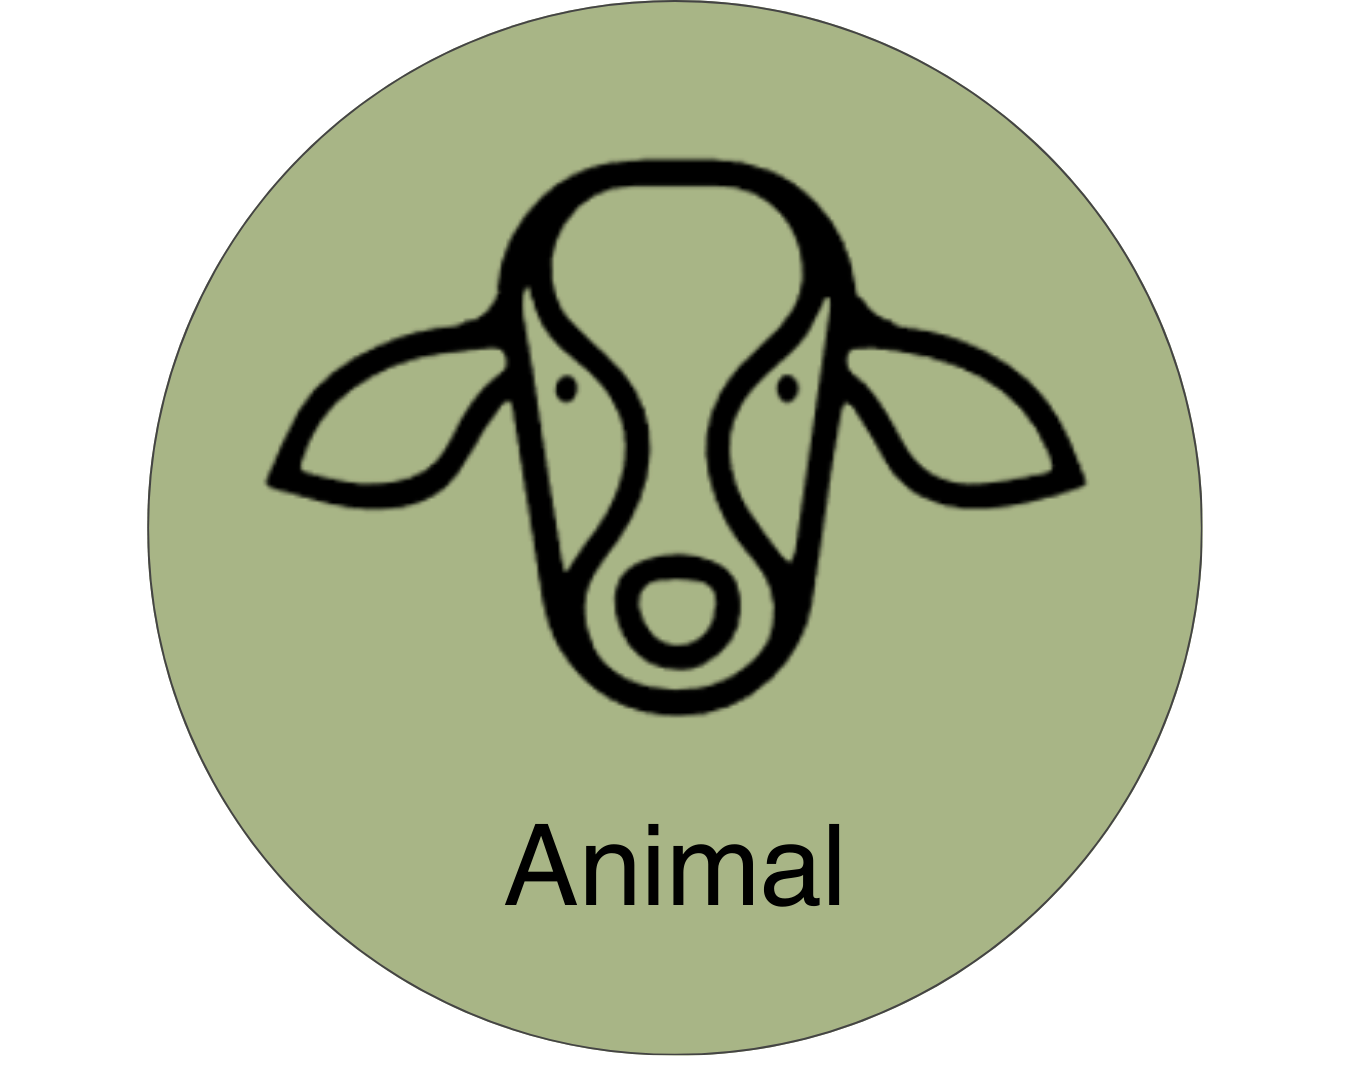
\includegraphics[width=0.35\linewidth,height=\textheight,keepaspectratio]{resources/animal.png}

}

\caption{\label{fig-animal-icon}Animal module icon}

\end{figure}%

\subsection{Example of a Table}\label{example-of-a-table}

\begin{longtable}[]{@{}ll@{}}
\caption{Example animal inputs}\label{tbl-animal-inputs}\tabularnewline
\toprule\noalign{}
Variable & Definition \\
\midrule\noalign{}
\endfirsthead
\toprule\noalign{}
Variable & Definition \\
\midrule\noalign{}
\endhead
\bottomrule\noalign{}
\endlastfoot
heiferI\_num & Number of Heifer I animals \\
\end{longtable}

\subsection{Examples of Equations}\label{examples-of-equations}

\protect\phantomsection\label{eqn-an-nrc-2}
\[ CBW = MW * 0.06275 \tag{\textbf{AN.NRC.2}}\]

\protect\phantomsection\label{eqn-an-nrc-3}
\[ CBW = MW * 0.06275 \tag{\textbf{AN.NRC.3}}\]

\protect\phantomsection\label{eqn-an-nrc-4}
\[ CBW = MW * 0.06275 \tag{\textbf{AN.NRC.4}}\]

\protect\phantomsection\label{eqn-an-nrc-5}
\[ CBW = MW * 0.06275 \tag{\textbf{AN.NRC.5}}\]

\protect\phantomsection\label{eqn-an-nrc-1}
\[ CBW = MW * 0.06275 \tag{\textbf{AN.NRC.1}}\]

\protect\phantomsection\label{eqn-an-nrc-2}
\[ CBW = MW * 0.06275 \tag{\textbf{AN.NRC.6}}\]

see (\textbf{eqn-an-nrc-2?})

\bookmarksetup{startatroot}

\chapter{Manure Module}\label{manure-module}

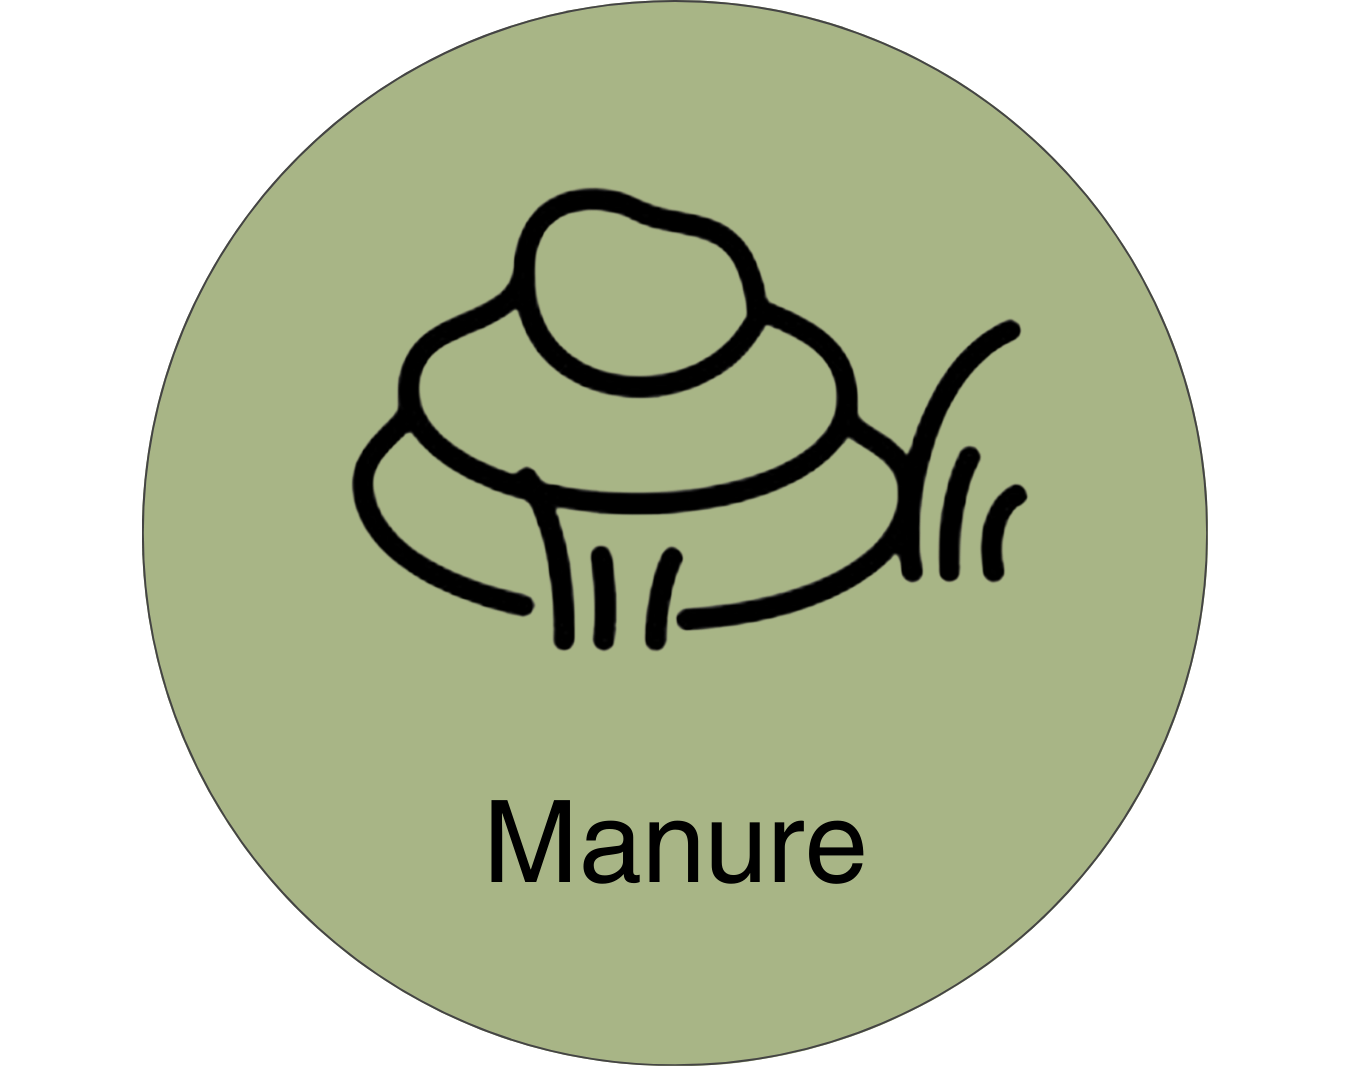
\includegraphics[width=1.45833in,height=\textheight,keepaspectratio]{resources/manure.png}

\section{Introduction}\label{introduction-1}

\subsection{Example of a Figure}\label{example-of-a-figure-1}

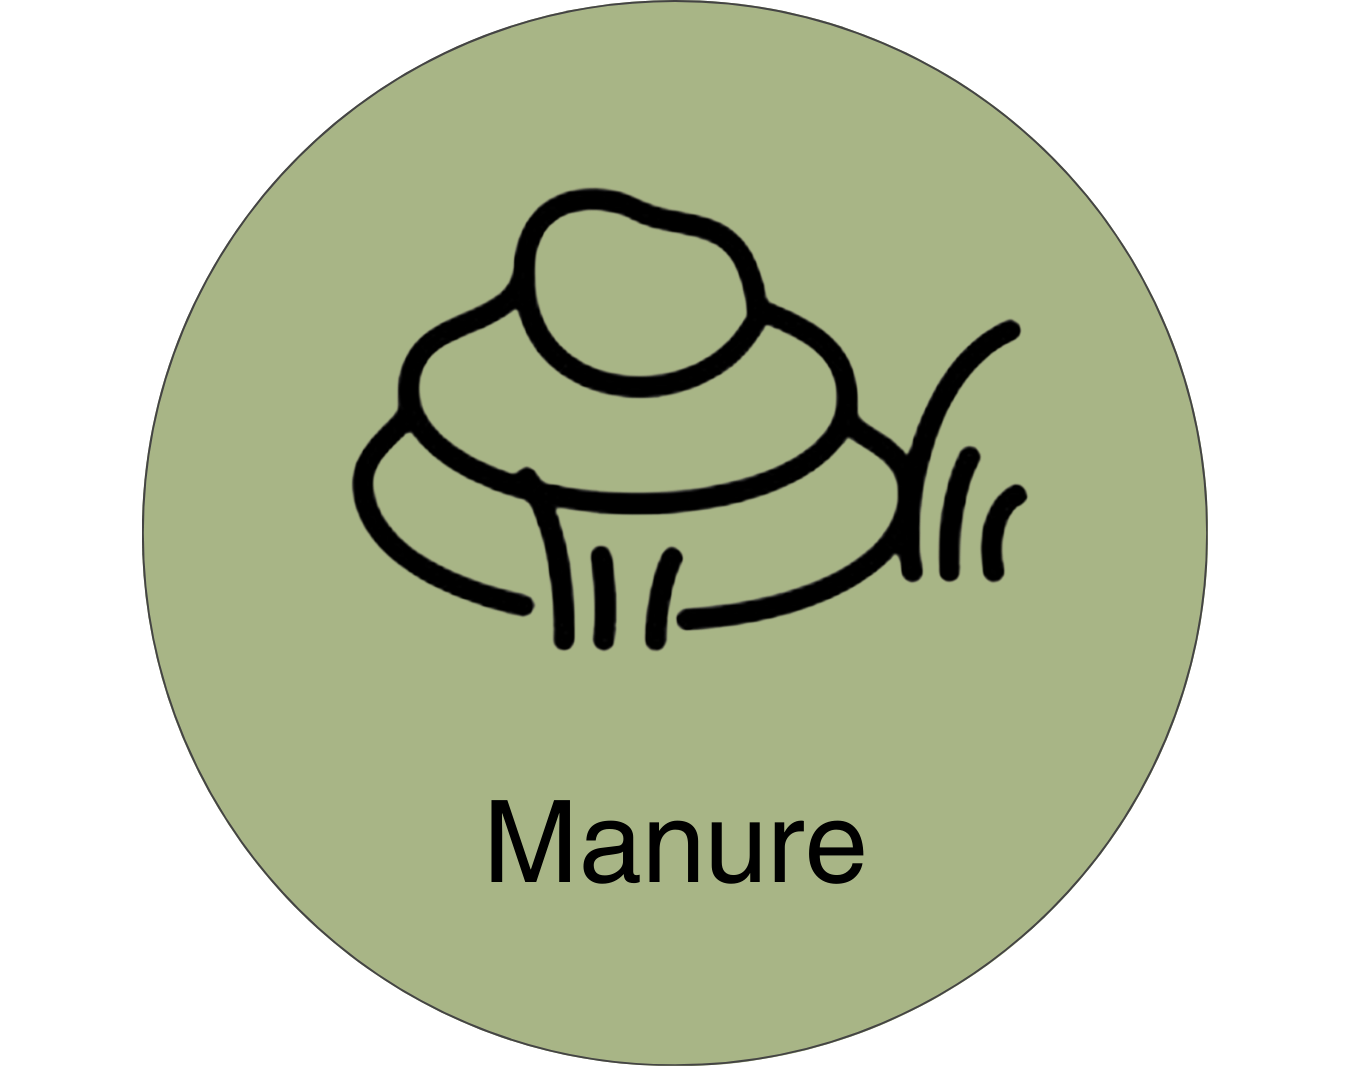
\includegraphics[width=0.5\linewidth,height=\textheight,keepaspectratio]{resources/manure.png}

\subsection{Example of a Table}\label{example-of-a-table-1}

\begin{longtable}[]{@{}ll@{}}
\caption{Example animal inputs}\label{tbl-animal-inputs}\tabularnewline
\toprule\noalign{}
Variable & Definition \\
\midrule\noalign{}
\endfirsthead
\toprule\noalign{}
Variable & Definition \\
\midrule\noalign{}
\endhead
\bottomrule\noalign{}
\endlastfoot
heiferI\_num & Number of Heifer I animals \\
\end{longtable}




\end{document}
